\section{データ間の特性}
本研究で電力使用量の予測に用いるデータは, 電力使用量, 天気, 気温, 降水量を用いる.
また, LSTM で入力としてこれらのデータを扱う場合に, データ間に関連性がない時に入力として適していないと考えられるので, データ間の相関関係として相関係数の計算を行う.

%%%%%%%%%%%%%%%%%%%%%%%%%%%%%%%%%%%%%%%%%%%%%%%%%%%%%%%%%%%%%%%%%%%%%%%%%%%%%%%%
\subsection{電力使用量}
東京電力パワーグリッド株式会社が提供している 2016 年 4 月から 2020 年 12 月までの東京電力が供給した電力使用量のデータであり, 年度, 日にち, 1 時間ごとの電力使用量(万 Kw)の3 要素が csv ファイルで提供されている.
2016 年は 4 月からのデータの公開のため, 6600rows * 3columns, 2017 年から 2019 年は 8760rows * 3columns, 2020 年は閏年であり通常よりも1日分多いため 24 列多い 8784rows * 3columns のデータである.
また, 用いるデータの一例を図 0 に示す.
これらのデータの日にちと時間を結合させて日時のデータとする. また, その際に日付と時間が並んでいるだけの文字列であるので, Python のデータ解析用ライブラリである pandas を用いて文字列を日付データに変換する.
また, データを可視化してグラフにしたものの例として 2019 年, 2020 年のグラフ及び,
2020 年 4 月の 5 日から 11 日, 12 日から 18 日, 19 日から 25 日の 3 週分のグラフをそれぞれ図に示す.

%%%%%%%%%%%%%%%%%%
\begin{figure*}[hb]
\centering
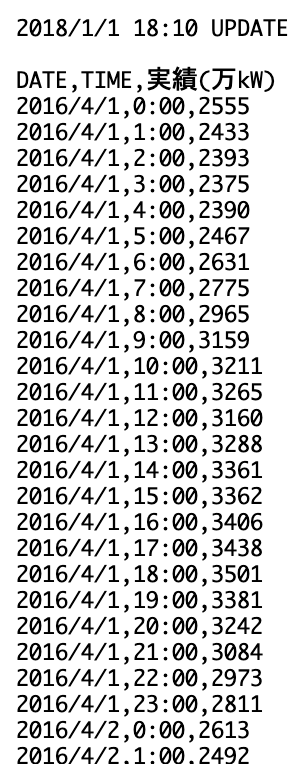
\includegraphics[scale=0.5]{exe_csv.png}
 \caption{用いる電力使用量データ例}
\end{figure*}
%%%%%%%%%%%%%%%%%%
%%%%%%%%%%%%%%%%%%
\begin{figure*}[hb]
  \centering
%  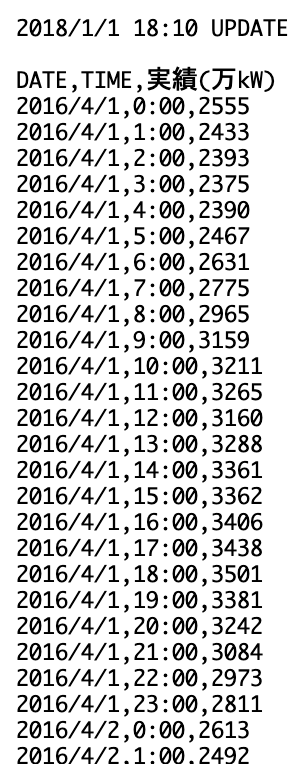
\includegraphics[scale=1.0]{exe_csv.png}
% \caption{用いる電力使用量データ例}
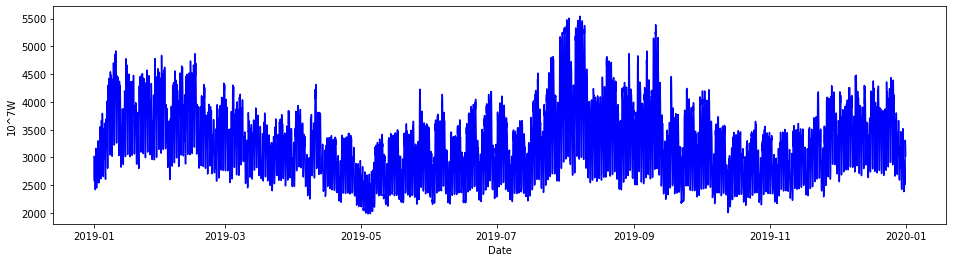
\includegraphics[scale=0.5]{2019_W.png}
 \caption{2019 年の電力使用量のグラフ}
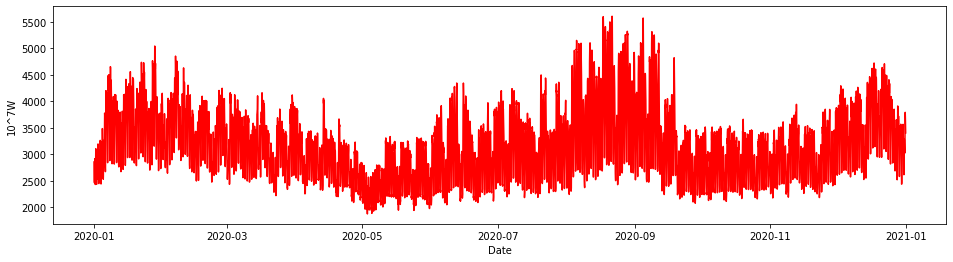
\includegraphics[scale=0.5]{2020_W.png}
 \caption{2020 年の電力使用量のグラフ}
\end{figure*}
%%%%%%%%%%%%%%%%%%
%%%%%%%%%%%%%%%%%%
%% \begin{figure*}[hb]
%% \centering
%% 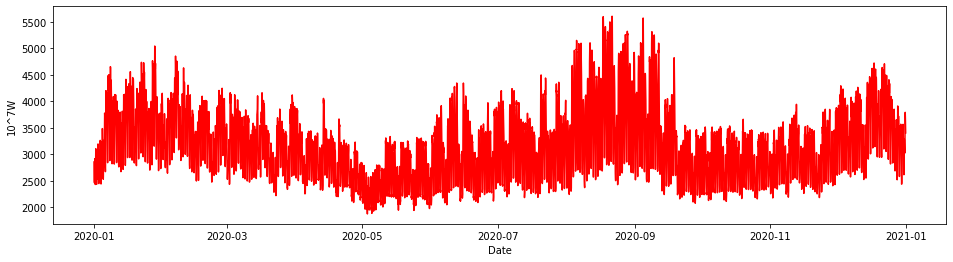
\includegraphics[scale=0.5]{2020_W.png}
%%  \caption{2020 年の電力使用量のグラフ}
%% \end{figure*}
%%%%%%%%%%%%%%%%%%

%%%%%%%%%%%%%%%%%%%%%%%%%%%%%%%%%%%%%%%%%%%%%%%%%%%%%%%%%%%%%%%%%%%%%%%%%%%%%%%%
\subsection{天気}

%%%%%%%%%%%%%%%%%%%%%%%%%%%%%%%%%%%%%%%%%%%%%%%%%%%%%%%%%%%%%%%%%%%%%%%%%%%%%%%%
\subsection{気温}

%%%%%%%%%%%%%%%%%%%%%%%%%%%%%%%%%%%%%%%%%%%%%%%%%%%%%%%%%%%%%%%%%%%%%%%%%%%%%%%%
\subsection{降水量}

\subsection{各データ間の相関係数}

数値計算を効率的に行うための拡張モジュールである, numpy を用いて相関係数を計算する.
相関係数は, 2 組のデータ間の関係性を示す指標の一つとして用いられているものである[Numpyデータ処理入門 p346〜].
相関係数を $r$ とすると $r$ は, $-1 ≦ r ≦ 1$ の範囲に値を取り, $r$ の絶対値が大きいほど, 大きい負の相関や正の相関を持つ.
例えば, 2 組のデータ, $X$ と $Y$ が存在しているとし, $X$ の分散を $V_X$, $Y$ の分散を $V_Y$ として, $X$ の標準偏差を $S_X$, $Y$ の標準偏差を $S_Y$ として, 共分散を $S_XY$ とおくと, 相関関係 $r$ は以下の式()で表される.

\begin{equation}
  r = S_{XY}/\sqrt{V_XV_Y} = S_{XY}/S_XS_Y
  \label{eq:corrcoef}
\end{equation}
